\include{algcomp_folha_header8}
\usepackage{hyperref}
\usepackage{graphicx}
\newcommand{\real}[1]{\underline{\mathbf{#1}}} 
\newcommand{\mod}{\mathrm{mod}\:}

\begin{document}
\writetitle{7.11.2011}{5}{5}


\nextsect

\sectitle{Parametrização}
\begin{enumerate}
\item[1] Mostre que $V=\{(x,y)\in \RR^2 \mid x \geq 0\}$ não é uma variedade afim.
\item[2] Seja $f\in \RR[x]$. Encontre uma parametrização de $V(y-f(x))$.
\end{enumerate}
\begin{tabular}{lr}
 \begin{minipage}{0.7\textwidth}
  \begin{enumerate}
    \item[3] Encontre uma parametrização da hiperbola $V(x^2-y^2-1)$ considerando a recta que une os pontos $(-1,0)$ e $(0,t)$. 
  \end{enumerate}
\vspace{4cm}
 \end{minipage}
&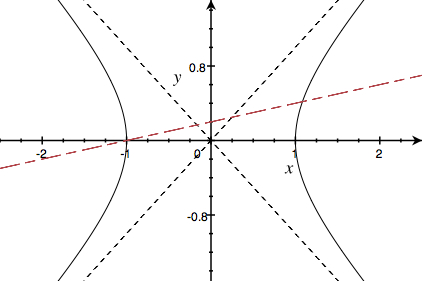
\includegraphics[width=4cm]{hiperbola.jpg}\\
\begin{minipage}{0.7\textwidth}
 \begin{enumerate}
  \item[4] Considere a curva $V=V(y^2-x^2-x^3)$:
  \begin{enumerate}
	\item Verifique que qualquer recta intersecta $V$ em $0$, $1$, $2$ ou $3$ pontos.
	\item Verifique que uma reta $y=mx$ intersecta $V$ em $(0,0)$ e exactamente mais um ponto se $m^2\neq 2$.
	\item Considerando a recta que une $(0,0)$ e $(1,t)$ encontre uma parametrização de $V$.
  \end{enumerate}
 \end{enumerate}\vspace{2cm}
\end{minipage}
&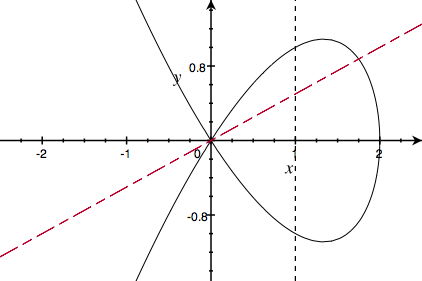
\includegraphics[width=4cm]{curva.jpg}
 \end{tabular}
 \begin{enumerate}
 \item[5] Encontre uma parametrização da espfera $S^2=V(x^2+y^2+z^2-1)$.
 \begin{enumerate}
 \item (Projeção estereográfica): Seja $(u,v,0)$ um ponto do plano $x,y$. Encontre uma parametrização da reta $L_{u,v}$ que une  o polo norte $(0,0,1)$ e o ponto $(u,v,0)$.
 \item Encontre o outro ponto $(x(u,v),y(u,v),z(u,v))$ da intersecção da recta $L_{u,v}$ com $S^2$.
 \item Qual ponto de $S^2$ não pertence a imagem da parametrização $\gamma: \RR^2 \rightarrow S^2$ dado por $\gamma(u,v)=(x(u,v), y(u,v), z(u,v))$?
 \end{enumerate}
 \end{enumerate}




\end{document}